\section{Deep Knowledge Tracing}
\label{sec:DKT}

\subsection{Knowledge Tracing Going Deep}

Knowledge tracing is a common task for educational data mining, with a goal towards accurately model the students' knowledge acquisition process. The conventional method, Bayesian Knowledge Tracing (BKT), keeps a binary state for each skill (i.e. knowledge component, or concept), either known or unknown. When a skill is not learned, by doing exercises on the skill, the student may have some probability to transition to the learned state. When answering a question on a certain skill, the student could get it wrong even when he already knows the skill (i.e. there exists a slip rate). And reversely, a student can get a question correct with luck, without knowing the skill, which corresponds to a guess rate. There have been various extentions to BKT, like modeling the forgetting process, and collapsing similar skills into one (since BKT tracks each skill separately, this kind of practice is trying to address the relations between skills).

There has been a quite influential work published in 2015, \textit{Deep Knowledge Tracing} \footnote{\textit{Deep Knowledge Tracing}, Chris Piech et al, NIPS 2015.} (DKT), which adopts an LSTM to model students' knowledge acquisition. Retrospectively speaking, LSTM is basically an upgraded version of BKT. Instead of having one binary state representation for each skill, LSTM uses a long vector of real numbers (which is normally more than the number of skills) to represent the knowledge state. By doing this, LSTM could capture complicated (and unfortunately, not very interpretable) relationships between different skills. The four gate layers in LSTM also closely resemble the key parameters in a BKT. The output gate, which reads out the hidden state vector to get an output (i.e. belief state on each skill), is a counterpart of slip and guess rate. The update gate, which scales the update value from the input, is like the acquisition rate. And the forget gate is literally modeling the forgetting of a knowledge component. In a nutshell, LSTM just upgrades the model of these processes from a single real number, to a layer of fully connected neural network. Therefore, we wouldn't be surprised to see DKT vastly outperforms BKT.

DKT can be simplified as a function approximator which takes a student's practice history (sequence of exercises he did, and whether he got each exercise correct or not) as input, and outputs the predictions (belief states) of the probability of getting each skill correct if presented as the next question.

\subsection{Implementing DKT}

DKT is a good modeling method for the student, i.e., a learned transition model of hidden knowledge states. This could be useful in various parts in our group's projects. Therefore, the first thing to do is implementing the model. 

Although there has already been several published DKT implementations, besides being a great opportunity to sort out all the subtlety like sequence padding and dropouts in LSTM, there are several other advantages of having our own implementation. First of all, our implementation is in Python, under the Tensorflow framework. Python is a friendly language for machine learning and data mining practices with its various powerful packages, and Tensorflow is a more flexible deep learning frame work, both of which provide convenience not presented in previous implementations. More importantly, our ultimate goal of DKT doesn't stop at getting a prediction metric on the test dataset, but to adopt it to do planning and data mining, thus calling an off-the-shelf LSTM cell from the framework won't work for us, since we won't be having access to the inner state of the LSTM that way. We need to implement the LSTM from scratch to better accustom to our goals. At last, since we have the full access to the model's structure, we made a small step forward of DKT by connecting the readout layer to the trainable initial state vector, which enables our DKT to predict the first answer without any previous input (which is a feature not presented in the original DKT implementation).

\subsection{Sanity Checks for DKT}

The biggest challenge of implementing a deep learning model is verifying the model. It requires little tuning (which is a great characteristic of using Adam optimizer in stochastic gradient descent) to get an AUC prediction performance comparable with previous works on the test set, however, we need more than a single AUC number to convince us that the model can be trusted.

Besides conventional checks like printing out or plotting several crucial variables/metrics, we did a more convincing sanity check. The goal is to test if DKT can fully recover a BKT model. First, we did a BKT simulation with 5 skills, each has its unique set of BKT parameters. As an extention to vanilla BKT, we add several prerequisite relations into the simulation: skill 0 and 1 are prerequisites for skill 2, while skill 2 and 3 are prerequisites for skill 4. We simulate such relations in a rather simplified manner: the student's acquisition rate of a skill would stay 0 until he learns all the prerequisites.

BKT model is actually a two-state HMM model, with acquisition rate corresponds to transition model, slip and guess rate corresponds to sensor model. Therefore, we can easily construct an oracle BKT inference model, which knows all the hidden parameters of BKT, and can infer the student's hidden knowledge state with the simulated trajectories as observations. A small tweak is needed to accustom to the prerequisite relations: the acquisition rate is an expected probability, conditioned on the knowledge states of prerequisites.

DKT can achieve the same AUC, 0.81, with this oracle BKT inference model. Again, only a AUC number won't be enough (there are millions of ways to accidentally get a high AUC). We computed the MSE (mean squared error) of the step-by-step belief states predicted by both models on the test set and got 0.003, which is a small number, but we still don't know if it's small enough. Therefore, we plot the knowledge tracing process given by the two models and compare the trends. From \ref{fig:match} we can see that DKT gives nearly identical predictions with oracle BKT. Combined with all the previous checks, we can safely say that our DKT model can be trusted and adopted in the projects.

\begin{figure}
\subfloat[DKT result on student 9999.]{
  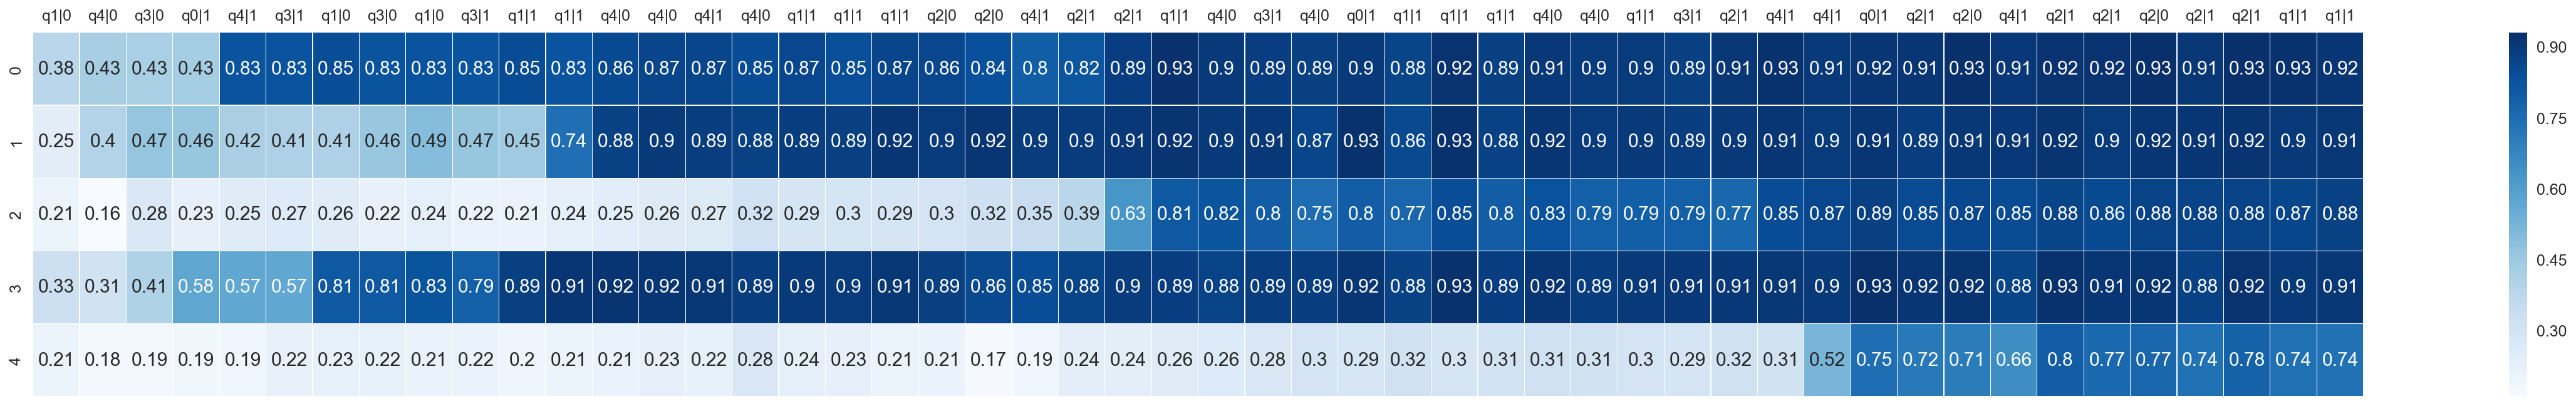
\includegraphics[width=1.0\linewidth]{figures/5th_dkt_9999.png}%
}
\newline
\subfloat[Oracle BKT result on student 9999.]{
  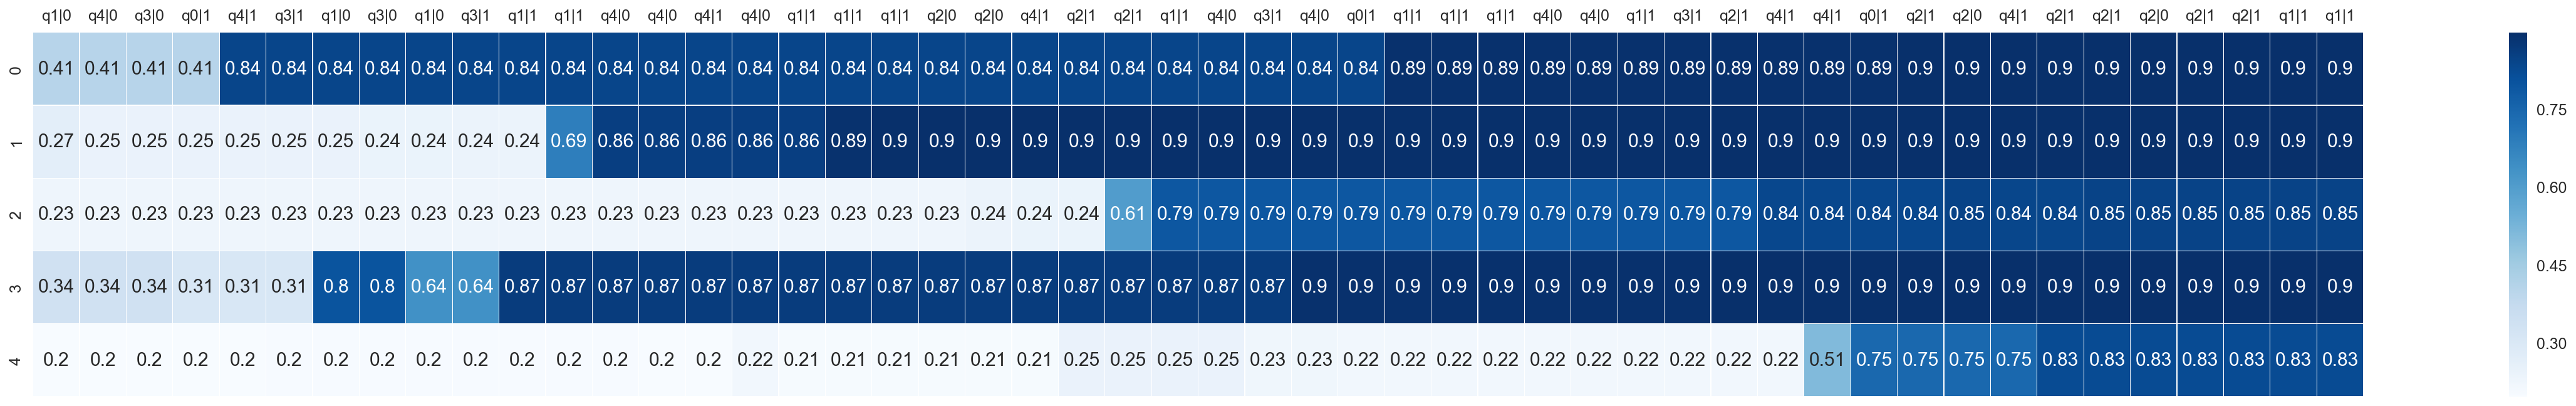
\includegraphics[width=1.0\linewidth]{figures/5th_bkt_9999.png}%
}
\caption{An example of the knowledge tracing visualization of DKT and BKT on one of the simualated student trajectory. The row labels are student ids. The column labels, $qi|j$, are student actions in each time step (with the leftmost action as the earliest): the question is on skill $i$, $j=1$ when the student answers correctly, otherwise $j=0$. Each column is the prediction for the action in the column label.}
\label{fig:match}
\end{figure}

In addition, we did a more novel sanity check, in which we reorder the train or test set in various ways and observe the consequenct AUC performance. This yields some interesting results and end up being a new project, which is ellaborated in section \ref{sec:influence}.
















